\documentclass[a4paper,11pt,table]{article}
%Import Packages %\[
\usepackage{fullpage}                                                   %This sets the margines to standard.
\usepackage{cancel}                                                     %This allows commands to put lines through terms.
\usepackage{mathtools}                                                  %This adds a series of packages designed to enhance the appearance of documents containing a lot of mathematics.
\usepackage{amsmath,amssymb,amsfonts,amsthm}                            %This adds many math commands.
\usepackage{setspace}                                                   %This allows for double or single spacing commands.
\usepackage{tikz}                                                       %This adds drawing features.
\usepackage{pgfplots}                                                   %This adds function plotting.
\usepackage{chngcntr}                                                   %This allows for convenient numbering.
\usepackage{fancyhdr}                                                   %This allows for a nice header.
\usepackage{caption}                                                    %This allows for custom captions.
\usepackage{listings}
\usepackage{graphicx}\graphicspath{{"figures"/}}                        %This allows the import and display of figures. %\]
%Renew Commands %\[
\renewcommand{\t}{\text}                                                %This is a shortcut for the text environment.
\renewcommand{\c}{\cdot}                                                %This is a shortcut for the dot operator.
\renewcommand{\sp}[1]{\left[#1\right]}                                  %This is a shortcut for hard brackets.
\renewcommand{\P}{\mathbb{P}}                                           %This is a shortcut for blackboard P.
\renewcommand{\l}{\ell}                                                 %This is a shortcut for script l.
\renewcommand{\rm}[1]{\begin{bmatrix*}[r] #1\end{bmatrix*}}             %This is a shortcut for a matrix.
\renewcommand{\i}{\overline{i}}                                         %This is a shortcut for i conjugate.
\renewcommand{\j}{\overline{j}}                                         %This is a shortcut for j conjugate.
\renewcommand{\k}{\overline{k}}                                         %This is a shortcut for k conjugate.
\renewcommand{\l}{\overline{l}}                                         %This is a shortcut for k conjugate.
\renewcommand{\r}{\scriptr}                                             %This is a shortcut for script r.%\]
%New Commands %\[
\newcommand*\rfrac[2]{{}^{#1}\!/_{#2}}                                  %This creates a one line fraction.
\newcommand{\ptl}[2]{\frac{\partial #1}{\partial #2}}                   %This is a shortcut for partials.
\newcommand{\sptl}[2]{\frac{\partial^2 #1}{\partial #2^2}}              %This is a shortcut for second partials.
\newcommand{\p}[1]{\left(#1\right)}                                     %This is a shortcut for parenthesis.
\newcommand{\hb}[1]{\left[#1\right]}                                    %This is a shortcut for hard brackets.
\newcommand{\set}[1]{\left\{#1\right\}}                                 %This is a shortcut for set notation.
\newcommand{\bra}[1]{\langle #1 |}                                      %This is a shortcut for bras.
\newcommand{\ket}[1]{| #1 \rangle}                                      %This is a shortcut for Kets.
\newcommand{\R}{\mathbb{R}}                                             %This is a shortcut for blackboard R.
\newcommand{\Z}{\mathbb{Z}}                                             %This is a shortcut for blackboard Z.
\newcommand{\N}{\mathbb{N}}                                             %This is a shortcut for blackboard N.
\newcommand{\C}{\mathbb{C}}                                             %This is a shortcut for blackboard C.
\newcommand{\Q}{\mathbb{Q}}                                             %This is a shortcut for blackboard C.
\newcommand{\comm}[2]{\left[#1, #2\right]}                               %This is a shortcut for the commutation operator.
\newcommand{\F}{\mathbb{F}}                                             %This is a shortcut for blackboard F.
\newcommand{\fa}{\forall}                                               %This is a shortcut for the upsidedown A symbol.
\newcommand{\m}[1]{\begin{bmatrix*}[r] #1\end{bmatrix*}}                %This is a shortcut for a matrix.
\newcommand{\cm}[1]{\begin{bmatrix*}[c] #1\end{bmatrix*}}               %This is a shortcut for a matrix.
\newcommand{\vm}[1]{\begin{vmatrix}#1\end{vmatrix}}                     %This is a shortcut for a matrix determinant.
\newcommand{\beq}{\begin{displaymath}}                                  %This is a shortcut for opening equation editor.
\newcommand{\eeq}{\end{displaymath}}                                    %This is a shortcut for closing equation editor.
\newcommand{\xhat}{\hat{x}}                                             %This is a shortcut for the x unit vector.
\newcommand{\yhat}{\hat{y}}                                             %This is a shortcut for the y unit vector.
\newcommand{\zhat}{\hat{z}}                                             %This is a shortcut for the z unit vector.
\newcommand{\Hhat}{\hat{H}}                                             %This is a shortcut for the Hamiltonian operator.
\newcommand{\del}{\v\nabla}                                             %This is a shortcut for the del operator.
\newcommand{\norm}[1]{\left|#1\right|}                                  %This is a shortcut for the norm operation.
\newcommand{\normsq}[1]{\left|#1\right|^2}                              %This is a shortcut for the norm operation.
\DeclarePairedDelimiter\ceil{\lceil}{\rceil}                            %This is a shortcut for the ceiling shorthand.
\DeclarePairedDelimiter\floor{\lfloor}{\rfloor}                         %This is a shortcut for the floor shorthand.
\newcommand{\bvec}[1]{\mathbf{#1}}                                      %This is a shortcut for a bold character. %\]
%New Definitions %\[
%\[                                                                     %This is for folding in Notepad++
\let\oldsqrt\sqrt                                                       %This redefines the sqrt function as oldsqrt.
\def\sqrt{\mathpalette\DHLhksqrt}                                       %This line and the ones following redefine the sqrt function to be prettier.
\def\DHLhksqrt#1#2{\setbox0=\hbox{$#1\oldsqrt{#2\,}$}%
    \dimen0=\ht0\advance\dimen0-0.2\ht0\setbox2%
    =\hbox{\vrule height\ht0 depth -\dimen0}{\box0\lower0.4pt\box2}}
\def\dbar{{\mathchar'26\mkern-12mu d}}                                  %This defines the inexact differential symbol.
%\]%\]
\usepackage{hyperref}       % Hyperlink
\hypersetup{
    colorlinks=true,
    linkcolor=blue,
    filecolor=magenta,      
    urlcolor=cyan,
}

%Header %\[
\pagestyle{fancy}
\fancyhf{}
\rhead{}
\chead{From Collectivism to Individualism: A Conservative Paradigm for Predicting Soccer Success}
\lhead{}
\renewcommand{\headrulewidth}{0.5pt}
\setlength{\headheight}{12pt}
%\]

\renewcommand{\section}[1]{\stepcounter{section}\noindent\textbf{\arabic{section}.~#1}\\}
\counterwithin{equation}{section}
\counterwithin{figure}{section}

\begin{document}
\section{Introduction}
Predicting the outcome of sports matches is one of the favorite topics for statisticians and gamblers alike. It is an interesting problem where the question of the respective importance of randomness ('luck') and determinism ('skill') is hotly debated. Of course, much importance also lies in the fact that successful predictions can lead to lots of money. For soccer, previous prediction methods mostly used team-level features based solely on the record of the team while neglecting individual skills. We hypothesize that individual skills are crucial to soccer and contain much information for predicting match outcomes which those other methods are not utilizing. Therefore, in this project, we sought to develop a machine learning strategy that predicts the outcomes of soccer matches based mainly on the individual attributes of the players on each team. \\
~\\
\section{Data Collection and Processing}
We have implemented a vast array of programs that facilitate the process of scraping data from different websites and then pre-processing and combining them to yield consistent datasets that can be used for machine learning.

Our novel approach uses as features the in-game stats from the Electronic Arts' celebrated game franchise FIFA, which were \href{http://www.espnfc.us/blog/espn-fc-united-blog/68/post/2959703/fifa-17-player-ratings-system-blends-advanced-stats-and-subjective-scouting}{painstakingly crafted by the experts}. Those numerical stats (1-100) measuring skills falling under broad categories (attacking, skill, movement, power, mentality, defending, and goalkeeping) were obtained from ``https://sofifa.com''. For practical reasons, we averaged over different positions in the team (forward, midfielder, defender, goalkeeper) all the skills falling under those categories. This was then combined with the records of matches (obtained from ``http://www.worldfootball.net'') to yield a dataset consisting of match outcomes and player stats. For this project, we focused on Premier League matches played in 2010-2017. After throwing away data entries plagued with various errors and difficulties, we ended up with a training set consisting of 2104 Premier League matches played in 2010-2017 minus the 2015-2016 season and a test set consisting of 273 matches played in the 2015-2016 season.

This was all done by writing a \href{https://github.com/TheLordBlarg/Soccer_Success/tree/master/codes/data_processing}{vast array of programs} that facilitate all the steps from scraping raw xml off of different websites to processing and combining them to yield consistent datasets that can be used for machine learning. The programs had to be able to match the date and the name of the player from a list of players and dates found from the records of matches and the player database. The date was simple enough to convert to the same format and then take the newest data set up to the date of the match. The name required more finesse. First, an exact match was searched. If that was not found, a match of each name individually, but not in the same order and not requiring the name number of names, was checked. In the rare event that this failed, a manual entry was requested of the user.\\
~\\
\section{Data Analysis Approach}
The first method that we used to analyze the dataset obtained by above procedure was Weka. We used various algorithms that were identified to be promising during our preliminary investigations. Specifically, those included three tree algorithms, three Bayesian algorithms, and two logistic regression algorithms.

Complementing the Weka, we decided to create our own machine learning implementation. Specifically, we wrote a \href{https://github.com/TheLordBlarg/Soccer_Success/blob/master/codes/machine_learning/msc_nn_hpc.py}{Python script} implementing a neural network with one hidden layer and three softmax output units each corresponding to the probability of the input data belonging to each class. The algorithm also uses 10-fold cross-validation with random partitioning of the dataset into training/validation sets, intentionally mirroring the Weka's approach. One thing of note is that we have normalized the data such that each attribute lies in the $[0,1]$ range (i.e. divided by 100). This seemed to improve the result significantly (increasing the classification accuray by 5-10\%), presumably due to the reduction of overflow errors. For Weka performance, it had no significant impact.

Finally, we sought to investigate the relative predictive power of each feature. This is not only interesting in its own right (we might be able to determine which skills are most relevant for soccer), it can also be a helpful aid for guiding machine learning implementation, in particular serving as a sanity-check for the approach. In order to measure this quantitatively, we wrote a \href{https://github.com/TheLordBlarg/Soccer_Success/blob/master/codes/feature_analysis/info_entropy.py}{Python script} that calculates, for each attribute, the maximum information gain that can be achieved by making a split along that attribute (cf. decision trees). \\
~\\
\section{Results}
As mentioned above, we used 2104 Premier League matches played in 2010-2017, minus the 2015-2016 season, as our training and cross-validation set. 273 matches played in the 2015-2016 season was set aside as the test set.

Table \ref{table1} shows the results of various Weka algorithms. Sadly, none of the algorithms performed significantly better than the ZeroR baseline, measured in terms of their 10-fold cross-validation accuracy. Logistic regression, which performed the best, only yielded a 3\% improvement over the baseline. Furthermore, its test accuracy was significantly lower than the CV-accuracy, indicating that the generalization is poor\footnote{Note, however that the ZeroR performance has dropped significantly for the test set. This may indicate some incidental structures in the data that might be interfering with the results.}.

\begin{center}
    \begin{tabular}{|c|c|c|c|}
        \hline
        Algorithm               &   Training accuracy  &   10-fold cross-validation accuracy  &   Test accuracy \\
        \hline
        ZeroR                   &   0.4644          &   0.4644      &   0.3919 \\
        \hline
        J48                     &   0.9439          &   0.3912      &   0.3993 \\
        \hline
        REPTree                 &   0.5741          &   0.4838      &   \cellcolor{red!25}0.4505 \\
        \hline
        RandomForest            &   \cellcolor{red!25}1.0000          &   0.4829      &   0.4396 \\
        \hline
        NaiveBayes              &   0.4049          &   0.3593      &   0.3773 \\
        \hline
        BayesNet                &   0.4967          &   0.4829      &   0.4432 \\
        \hline
        NaiveBayesMultinomial   &   0.4316          &   0.4335      &   0.4029 \\
        \hline
        Logistic                &   0.5318          &   \cellcolor{red!25}0.4948      &   0.4286 \\
        \hline
        SimpleLogistic          &   0.5119          &   0.4924      &   0.4139 \\
        \hline
    \end{tabular}
    \captionof{table}{Training and 10-fold cross-validation accuracies for Premier League matches in 2010-2017. 2015-2016 season data was set aside as the test set to derive the test accuracy. The highest accuracy in each column has been shaded in light red. \label{table1}}
\end{center}

Our custom single hidden layer neural network implementation was no more successful. Figure \ref{figLC} shows the learning curve of the network with 30 hidden units. It is clear that there is underfitting and the model is incapable of capturing the underlying trend of the data. Same results were obtained for hidden layer size ranging from 10-100 units (see Figure \ref{figCVH}). This suggests that either the neural network architecture considered is insufficient (for instance, more than one hidden layers may be necessary) or the problem lies with the dataset itself.
\clearpage~\\
\begin{center}
    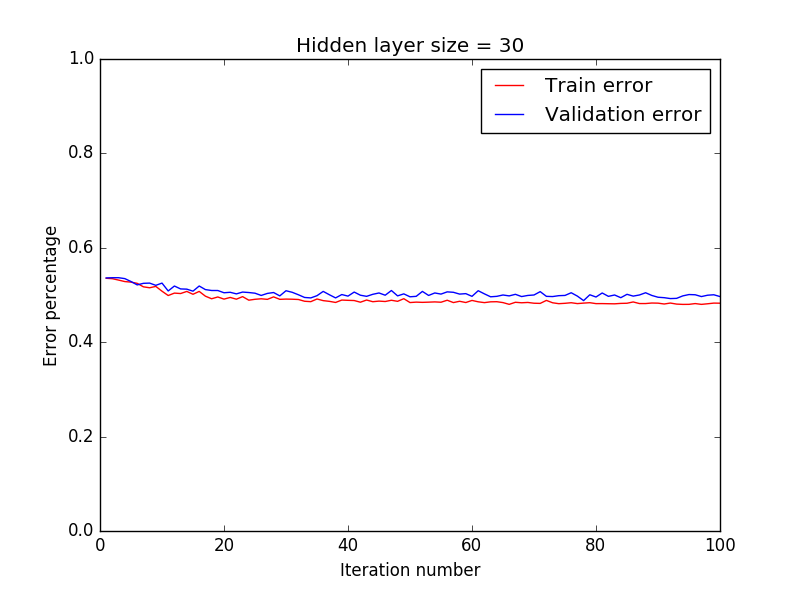
\includegraphics[scale=0.5]{learning_curve}
    \captionof{figure}{\label{figLC}}
    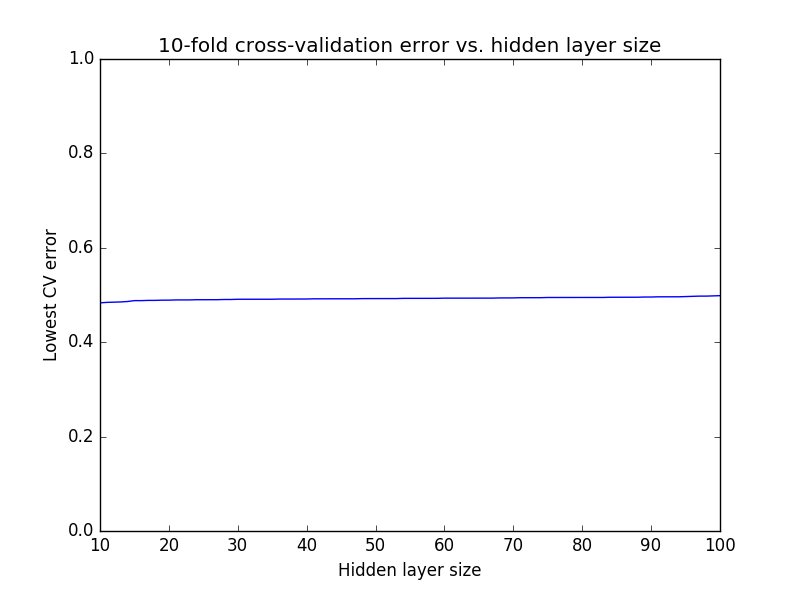
\includegraphics[scale=0.5]{CV_H}
    \captionof{figure}{\label{figCVH}}
\end{center}

Finally, Table \ref{tablefeature} lists select features and the corresponding information gain that can be obtained by making a split over the feature. Full data is available \href{https://github.com/TheLordBlarg/Soccer_Success/blob/master/results/entropy_train.csv}{in the repository}. A cursory glance suggests that skills related to goalkeeping and defending are the most important factors in deciding the outcome of a soccer match. However, this result should be taken with a grain of salt as there are also nonsensical results such as the goalkeeper's attacking or the forward's goalkeeping skills (which should be completely irrelevant to the match) yielding more information than defender's defending skills (which is clearly relevant). Though, this result is expected. It is predicted that Manchester City could've won the Premier League this year by a wide margin if they had David De Gea in goal instead of Claudio Bravio.

\begin{center}
    \begin{tabular}{|c|c|c|}
        \hline
        No. &   Attribute                           &   Information gain \\
        \hline
        1   &   Home Team; Goalkeeper; Goalkeeping  &   0.03567655 \\
        \hline
        2   &   Away Team; Goalkeeper; Goalkeeping  &   0.024776643 \\
        \hline
        3   &   Home Team; Defender; Defending      &   0.013332217 \\
        \hline
        4   &   Home Team; Goalkeeper; Movement     &   0.013321315 \\
        \hline
        5   &   Home Team; Defender; Movement       &   0.011140302 \\
        \hline
        \vdots  &   \vdots  &   \vdots \\
        \hline
        37  &   Home Team; Goalkeeper; Attacking    &   0.003304952 \\
        \hline
        \vdots  &   \vdots  &   \vdots \\
        \hline
        43  &   Away Team; Goalkeeper; Attacking    &   0.002832013 \\
        \hline
        \vdots  &   \vdots  &   \vdots \\
        \hline
        51  &   Home Team; Forward; Goalkeeping     &   0.002177446 \\
        \hline
        52  &   Away Team; Forward; Goalkeeping     &   0.002115403 \\
        \hline
        53  &   Away Team; Defender; Defending      &   0.00206549 \\
        \hline
    \end{tabular}
    \captionof{table}{A selection of attributes listed in the order of decreasing information gain (in bits). Prior entropy is 1.5305276569. \label{tablefeature}}
\end{center}
~\\
\section{Discussion}
While the results were not as good as one would hope, they still are a promising start. There was a performance gain over ZeroR that was noticeable over large datasets. Our data was averaging over players and therefor was still crude in this respect. Furthermore, only simple models were fit to the data. For example, models that predicted probabilities of a team getting a win, draw, or loss would be more appropriate than a model that simply predicted it outright.

Finally, it may be the case that although individual attributes alone do not have enough predictive power, combining them with team-based features can yield drastically improved performance that cannot be achieved by using either set of features alone. This would be the natural direction to explore in any future work. \\

~\\
\section{Acknowledgements}
Jeremy Rath worked mainly on data collection and processing. Hyun Jin Kim worked mainly on data analysis. Both authors worked on setting up the webpage and preparing this report.

~\\
\end{document}
